\documentclass[10pt,a4paper]{article}
\usepackage[margin=0.5in]{geometry}
\usepackage[utf8]{inputenc}
\usepackage[english]{babel}
\usepackage{amsmath}
\usepackage{amsfonts}
\usepackage{amssymb}
\usepackage{cancel}
\usepackage{xcolor}
\usepackage{graphicx}
\usepackage{hyperref}


%\renewcommand\CancelColor{<color command>}
\newcommand\cc[2][black]{\renewcommand\CancelColor{\color{#1}}\cancel{#2}}
\newcommand{\ud}[1]{\underline{#1}}
\DeclareMathOperator{\tm}{\times}
\DeclareMathOperator{\cross}{\wedge}
\DeclareMathOperator{\A}{\ud{A}}
\DeclareMathOperator{\B}{\ud{B}}
\DeclareMathOperator{\C}{\ud{C}}
\DeclareMathOperator{\D}{\ud{D}}
\DeclareMathOperator{\E}{\ud{E}}
\DeclareMathOperator{\AB}{\ud{AB}}
\DeclareMathOperator{\DA}{\ud{DA}}
\DeclareMathOperator{\AD}{\ud{AD}}
\DeclareMathOperator{\DB}{\ud{DB}}
\DeclareMathOperator{\BD}{\ud{BD}}
\DeclareMathOperator{\ED}{\ud{ED}}
\DeclareMathOperator{\EA}{\ud{EA}}
\DeclareMathOperator{\EB}{\ud{EB}}
\DeclareMathOperator{\DE}{\ud{DE}}
\DeclareMathOperator{\DC}{\ud{DC}}
\DeclareMathOperator{\CA}{\ud{CA}}
\DeclareMathOperator{\OA}{\ud{OA}}
\DeclareMathOperator{\z}{\ud{z}}
\DeclareMathOperator{\e}{\ud{e}}
\DeclareMathOperator{\n}{\ud{n}}
\DeclareMathOperator{\en}{\ud{e}\cdot\ud{n}}
\DeclareMathOperator{\OEz}{\|\ud{OE} \cross \z\|}
\DeclareMathOperator{\OEn}{\|\ud{OE}\|}
\DeclareMathOperator{\c1}{(l^2 + 2l\OA\cdot\e)}


% \DeclareMathOperator{\cn}{\mathbf{c}}


\title{Find reflexion points on a a 3d surface}
\begin{document}

\maketitle


\tableofcontents
\newpage

% 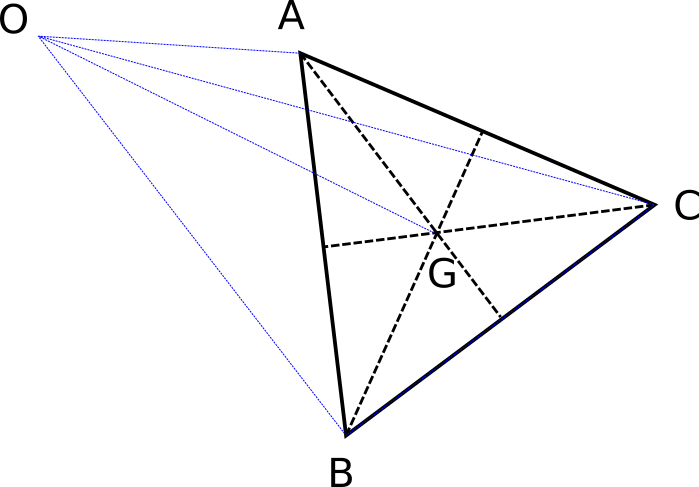
\includegraphics[scale=0.4]{tetra.png} 


\section{Notations}

\begin{itemize}
    \item $\A$ is the point of observation
    \item $\B$ is the point observed
    \item $\C$ is the local coordinate center of the 3d surface
    \item $\D$ is the projection of $\B$ on the 3d surface as seen from $\A$
    \item $\e$ is the unit vector such that $\AB = \|\AB\|\e = l\e$
    \item $\E$ is a point on $(AB)$ parameterized by $\ud{AE} = kl\e$
    \item $\n(D)$ is the normal vector of the 3d surface at point $\D$
\end{itemize}


Point $\D$ on the 3d sufarce is the reflexion point connecting $A$ and $B$.
It means that $\n(D)$ is in the same plane as $(A, D, B)$.

Point $\E$ on is the projection, on line $(A, B)$ of point $\D$ along $\n$.


The idea is to look for $\E$, which is parameterized by $k$, and then derive
$\D$ from $\E$.

Hence both $\n(\D)$ and $d_E = \|\ED\|$ are parametrized by $k$:
$\n(k)$ and $d_E(k)$.


\newpage
\section{General equations}

\subsection{co-planarity}

The point $\D$ on the 3d sufarce is such that $\n(D)$ is in the same plane as
$(A, D, B)$, which is written:

\begin{equation}
( \DA \cross \n ) \cdot ( \DB \cross \n ) = 0
\end{equation}


$$
\begin{array}{lll}
    & ( \DA \cross \n ) \cross ( \DB \cross \n ) = 0\\
    \Leftrightarrow
    & ( \EA \cross \n ) \cross ( \EB \cross \n ) = 0\\
    & ( (-kl)\e \cross \n ) \cross ( (1-k)le \cross \n ) = 0\\
    & k(1-k)l^2(\e \cross \n) \cross (\e \cross \n) = 0\\
\end{array}
$$

Which is true by construction of $E$.

\subsection{equal angles}

Since it is a specular reflexion, angles $(A,D,E)$ and $(B,D,E)$ are equal,
which means $\E$ is necessarily standing on the bisector of angle $(A, D, B)$.

As such, the distance between $\E$ and line $(A, D)$ is equal to the distance
between $\E$ and line $(B, D)$, which is written:

$$
d_{E,(A,D)}
= \frac{\| \AD \cross \ud{AE} \|}{\| \AD \|}
= \frac{\| \BD \cross \ud{BE} \|}{\| \BD \|}
= d_{E,(B,D)}
$$

Knowing that:
$$
\begin{array}{lll}
    \| \AD \|^2
    & = \| \ud{AE} + \ED \|^2\\
    & = k^2l^2 + d_E^2 + 2\ud{AE} \cdot \ED\\
    & = k^2l^2 + d_E^2 + 2 kl\e \cdot (-d_E)\n\\
    & = k^2l^2 + d_E(k)^2 - 2 kld_E(k) \e \cdot \n(k)
\end{array}
$$

Similarly:
$$
\begin{array}{lll}
    \| \BD \|^2
    & = \| \ud{BE} + \ED \|^2\\
    & = (1-k)^2l^2 + d_E^2 + 2\ud{BE} \cdot \ED\\
    & = (1-k)^2l^2 + d_E^2 + 2 (1-k)l(-\e) \cdot (-d_E)\n\\
    & = (1-k)^2l^2 + d_E(k)^2 + 2 (1-k)ld_E(k) \e \cdot \n(k)
\end{array}
$$

And the cross-products:
$$
\begin{array}{lll}
    \| \AD \cross \ud{AE} \|^2
    & = \| \ED \cross \ud{AE} \|^2\\
    & = \| (-d_E)\n \cross kl\e \|^2\\
    & = k^2d_E(k)^2l^2 \| \n(k) \cross \e \|^2\\
\end{array}
$$

And:
$$
\begin{array}{lll}
    \| \BD \cross \ud{BE} \|^2
    & = \| \ED \cross \ud{BE} \|^2\\
    & = \| (-d_E)\n \cross (1-k)l(-\e) \|^2\\
    & = (1-k)^2d_E(k)^2l^2 \| \n(k) \cross \e \|^2\\
\end{array}
$$

So in the end:
$$
\begin{array}{lll}
    & d_{E, (A,D)}^2 = d_{E, (B,D)}^2\\
    \Leftrightarrow &
    \| \AD \cross \ud{AE} \|^2 \| \BD \|^2
    = \| \BD \cross \ud{BE} \|^2 \| \AD \|^2\\
    \Leftrightarrow &
    k^2d_E^2l^2 \| \n \cross \e \|^2
    \left[ (1-k)^2l^2 + d_E^2 + 2 (1-k)ld_E \en \right]\\
    & = (1-k)^2d_E^2l^2 \| \n \cross \e \|^2
    \left[ k^2l^2 + d_E^2 - 2 kld_E \en \right]\\
\end{array}
$$

So assuming that:
$$
\left\{
    \begin{array}{ll}
        \| \n(k) \cross \e \| \neq 0\\
        l \neq 0\\
        d_E(k) \neq 0
    \end{array}
\right.
$$

So in the end:
$$
\begin{array}{lll}
    & d_{E, (A,D)}^2 = d_{E, (B,D)}^2\\
    \Leftrightarrow &
    k^2 \left[ (1-k)^2l^2 + d_E^2 + 2 (1-k)ld_E \en \right]
    = (1-k)^2 \left[ k^2l^2 + d_E^2 - 2 kld_E \en \right]\\
    \Leftrightarrow &
    k^2 \left[ d_E^2 + 2 (1-k)ld_E \en \right]
    = (1-k)^2 \left[ d_E^2 - 2 kld_E \en \right]\\
    \Leftrightarrow &
    k^2d_E^2 + 2 k^2(1-k)ld_E \en
    = (1-k)^2d_E^2 - 2(1-k)^2kld_E \en\\
    \Leftrightarrow &
    2kd_E^2 - d_E^2 + 2k(1-k)ld_E\en(k + 1 - k) = 0\\
    \Leftrightarrow &
    (2k - 1)d_E + 2k(1-k)l\en = 0\\
\end{array}
$$

Hence:
$$
(2) \Leftrightarrow (2k - 1)d_E(k) + 2k(1-k)l\en(k) = 0\\
$$

\newpage
\subsection{equal angles 2}

This time we use the scalar product:
$$
    (\DA\cdot\n)^2 \|DB\|^2 = (\DB\cdot\n)^2 \|DA\|^2
$$

With:
$$
\left\{
\begin{array}{ll}
    \DA\cdot\n = d - kl\en\\
    \DB\cdot\n = d + (1-k)l\en\\
    \|\DA\|^2 = d^2 + k^2l^2 - 2dkl\en\\
    \|\DB\|^2 = d^2 + (1-k)^2l^2 + 2d(1-k)l\en\\
\end{array}
\right.
$$

So:
$$
\begin{array}{ll}
    & (\DA\cdot\n)^2 \|DB\|^2 = (\DB\cdot\n)^2 \|DA\|^2\\
    \Leftrightarrow &
    (d - kl\en)^2 (d^2 + (1-k)^2l^2 + 2d(1-k)l\en)
    = (d - kl\en + l\en)^2 (d^2 + k^2l^2 - 2dkl\en)\\
    \Leftrightarrow &
    (d - kl\en)^2 ((1-k)^2l^2 + 2d(1-k)l\en - k^2l^2 + 2dkl\en)
    = (l^2\en^2 + 2l\en(d - kl\en))(d^2 + k^2l^2 - 2dkl\en)\\
    \Leftrightarrow &
    (d - kl\en)^2 (l^2 - 2kl^2 + 2dl\en)
    = l\en(l\en + 2d - dkl\en)(d^2 + k^2l^2 - 2dkl\en)\\
    \Leftrightarrow &

\end{array}
$$


\newpage
\section{Planar}

If the 3d surface is a plane, then $\n$ is constant and does not depend on $k$.

The equations become:

\begin{equation}
    (2k - 1)d_E(k) + 2k(1-k)l\en = 0\\
\end{equation}

In that case:
$$
\begin{array}{ll}
    d_E(k)
    & = \DE \cdot \n\\
    & = \left( \DC + \CA + \ud{AE} \right) \cdot \n\\
    & = \CA \cdot \n + kl \en\\
\end{array}
$$

Which means:
$$
\begin{array}{ll}
    (2)
    & \Leftrightarrow
    2k(\CA \cdot \n + kl\en) - \CA \cdot \n - kl \en + 2k(1-k)l\en = 0\\
    & \Leftrightarrow
    k^2(2l\en - 2l\en) + k(2\CA \cdot \n - l\en + 2l\en) - \CA \cdot \n = 0\\
    & \Leftrightarrow
    k(2\CA \cdot \n + l\en) - \CA \cdot \n = 0\\
\end{array}
$$

So finally:
$$
(2) \Leftrightarrow k = \frac{\CA \cdot \n}{2\CA \cdot \n + l\en}
$$

\newpage
\section{Cylinder}

Consider a cylinder of axes $(O, \z)$, with $\z$  unit vector and radius $r$.
The normal vector associated to any point $E$ (not on the axis) is:

$$
\n(E) = - \frac{(\ud{OE} \cross  \z) \cross \z}{
    \|(\ud{OE} \cross  \z) \cross \z\|
}
    = - \frac{(\ud{OE} \cross  \z) \cross \z}{\OEz}
$$

Given that $E$ in on the $(A, B)$ line:

$$
\ud{OE} = \ud{OA} + kl\e
$$

So:

$$
(\ud{OE} \cross \z) \cross \z
= (\ud{OA} \cross \z) \cross \z + kl( \e \cross \z )\cross \z
$$

Which entails:
$$
\begin{array}{ll}
    \en(k)
    & = - \frac{1}{\OEz}\left[ \e \cdot ((\ud{OE}\cross\z) \cross \z)\right]\\
    & = - \frac{1}{\OEz}\left[ \z \cdot (\e \cross (\ud{OE}\cross\z))\right]\\
\end{array}
$$

And:

$$
d_E = r - \OEz
$$

So the equation becomes:
$$
\begin{array}{ll}
    (2)
    & \Leftrightarrow
    (2k-1)(r - \OEz) + 2k(1-k)l\en = 0\\
    & \Leftrightarrow
    (2k-1)(r - \OEz)\OEz
    - 2k(1-k)l\left[ \z \cdot (\e \cross (\ud{OE}\cross\z))\right] = 0\\
    & \Leftrightarrow
    (2k-1)r\OEz - (2k-1)\OEz^2
    - 2k(1-k)l\left[ (\ud{OE}\cross\z) \cdot (\z \cross \e)\right] = 0\\
\end{array}
$$

Observing that:
$$
\ud{OE}\cross\z = \OA \cross \z + kl \e \cross \z
$$

And:
$$
\OEz^2 = \|\OA\cross\z + kl\e\cross\z\|^2
= (\OA\cross\z)^2 + 2kl(\OA\cross\z)\cdot(\e\cross\z) + k^2l^2(\e\cross\z)^2
$$

So 
$$
\begin{array}{llll}
    (2)
    & \Leftrightarrow &
    (2k-1)r\OEz
    - (2k-1)(\OA\cross\z)^2
    - (2k-1)2kl(\OA\cross\z)\cdot(\e\cross\z)
    - (2k-1)k^2l^2(\e\cross\z)^2\\
    &&- 2k(1-k)l(\ud{OA}\cross\z) \cdot (\z \cross \e) 
    - 2k^2(1-k)l^2(\e\cross\z) \cdot (\z \cross \e) & = 0\\
    & \Leftrightarrow &
    (2k-1)r\OEz
    - (2k-1)(\OA\cross\z)^2
    + 2kl(\OA\cross\z)\cdot(\e\cross\z)(1 - k - 2k + 1)
    + k^2l^2(\e\cross\z)^2(2 - 2k - 2k + 1) & = 0\\
    & \Leftrightarrow &
    (2k-1)r\OEz
    - (2k-1)(\OA\cross\z)^2
    + 2kl(\OA\cross\z)\cdot(\e\cross\z)(2 - 3k)
    + k^2l^2(\e\cross\z)^2(3 - 4k) & = 0\\
\end{array}
$$


\newpage
\section{Sphere}

Consider a sphere of center $O$ and radius $r$.
The normal vector associated to any point $E$ (not on $O$) is:

$$
\n(E) = - \frac{\ud{OE}}{\OEn}
$$

Given that $E$ in on the $(A, B)$ line:

$$
\left\{
\begin{array}{ll}
    \ud{OE} = \OA + kl\e\\
    \|\ud{OE}\|^2 = \|\OA\|^2 + k^2l^2 + 2kl\OA\cdot\e
\end{array}
\right.
$$

Which entails:
$$
\begin{array}{ll}
    \en(k)
    & = - \frac{1}{\OEn}\left[ \OA \cdot \e  + kl \right]\\
\end{array}
$$

And:

$$
d_E = r - \|\ud{OE}\|
$$

So the equation becomes:
$$
\begin{array}{llll}
    (2)
    & \Leftrightarrow &
    (2k-1)(r - \OEn) + 2k(1-k)l\en = 0\\
    & \Leftrightarrow &
    (2k-1)(r - \OEn)\OEn
    - 2k(1-k)l\left[ \OA \cdot \e  + kl \right] = 0\\
    & \Leftrightarrow &
    (2k-1)r\OEn - (2k-1)\OEn^2
    - 2k(1-k)l\OA\cdot\e  - 2k^2l^2(1-k) = 0\\
    & \Leftrightarrow &
    (2k-1)r\OEn - (2k-1)\|\OA\|^2 - (2k-1)k^2l^2 - 2(2k-1)kl\OA\cdot\e
    - 2k(1-k)l\OA\cdot\e  - 2k^2l^2(1-k) = 0\\
    & \Leftrightarrow &
    (2k-1)r\OEn - (2k-1)\|\OA\|^2 - k^2l^2(2k-1 + 2 - 2k)
    - 2kl\OA\cdot\e(2k-1 + 1 - k) = 0\\
    & \Leftrightarrow &
    (2k-1)r\OEn - (2k-1)\|\OA\|^2 - k^2l^2 - 2k^2l\OA\cdot\e = 0\\
    & \Leftrightarrow &
    (2k-1)^2r^2\OEn^2 = \left[ (2k-1)\|\OA\|^2 + k^2\c1 \right]^2\\
    & \Leftrightarrow &
    (2k-1)^2r^2\|\OA\|^2 + (2k-1)^2r^2k^2l^2 + (2k-1)^2r^2 2kl\OA\cdot\e\\
    & &= (2k-1)^2\|\OA\|^4 + 2(2k-1)\|\OA\|^2k^2\c1 + k^4\c1^2\\
    & \Leftrightarrow &
    (2k-1)^2(r^2 - \|\OA\|^2)\|\OA\|^2 + (2k-1)^2r^2k^2l^2 + (2k-1)^2r^2 2kl\OA\cdot\e\\
    & &= 2(2k-1)l\|\OA\|^2k^2(l + 2\OA\cdot\e)
    + k^4l^2(l + 2\OA\cdot\e)^2\\
    & \Leftrightarrow &
    (4k^2 - 2k + 1)C_0
    + (4k^2 - 2k + 1)k^2C_1
    + (4k^2 - 2k + 1)kC_2
    = (2k-1)k^2C_3 + k^4C_4\\ 
    & \Leftrightarrow &
    k^4\left[ 4C_1 - C_4 \right]
    + k^3\left[ -2C_1 + 4C_2 - 2C_3  \right]
    + k^2\left[ 4C_0 + C_1 - 2C_2  + C_3 \right]
    + k\left[ -2C_0 + C_2 \right]
    + C_0 = 0
\end{array}
$$

Where:
$$
\left\{
\begin{array}{llll}
    C_0 = (r^2 - \|\OA\|^2)\|\OA\|^2\\
    C_1 = r^2l^2\\
    C_2 = 2lr^2\OA\cdot\e\\
    C_3 = 2l\|\OA\|^2(l + 2\OA\cdot\e)\\
    C_4 = l^2(l + 2\OA\cdot\e)^2
\end{array}
\right.
$$

\newpage
\section{Toroidal}

\end{document}


